% Options for packages loaded elsewhere
\PassOptionsToPackage{unicode}{hyperref}
\PassOptionsToPackage{hyphens}{url}
\PassOptionsToPackage{dvipsnames,svgnames,x11names}{xcolor}
%
\documentclass[
]{article}
\usepackage{amsmath,amssymb}
\usepackage{iftex}
\ifPDFTeX
  \usepackage[T1]{fontenc}
  \usepackage[utf8]{inputenc}
  \usepackage{textcomp} % provide euro and other symbols
\else % if luatex or xetex
  \usepackage{unicode-math} % this also loads fontspec
  \defaultfontfeatures{Scale=MatchLowercase}
  \defaultfontfeatures[\rmfamily]{Ligatures=TeX,Scale=1}
\fi
\usepackage{lmodern}
\ifPDFTeX\else
  % xetex/luatex font selection
\fi
% Use upquote if available, for straight quotes in verbatim environments
\IfFileExists{upquote.sty}{\usepackage{upquote}}{}
\IfFileExists{microtype.sty}{% use microtype if available
  \usepackage[]{microtype}
  \UseMicrotypeSet[protrusion]{basicmath} % disable protrusion for tt fonts
}{}
\makeatletter
\@ifundefined{KOMAClassName}{% if non-KOMA class
  \IfFileExists{parskip.sty}{%
    \usepackage{parskip}
  }{% else
    \setlength{\parindent}{0pt}
    \setlength{\parskip}{6pt plus 2pt minus 1pt}}
}{% if KOMA class
  \KOMAoptions{parskip=half}}
\makeatother
\usepackage{xcolor}
\usepackage[margin=1in]{geometry}
\usepackage{color}
\usepackage{fancyvrb}
\newcommand{\VerbBar}{|}
\newcommand{\VERB}{\Verb[commandchars=\\\{\}]}
\DefineVerbatimEnvironment{Highlighting}{Verbatim}{commandchars=\\\{\}}
% Add ',fontsize=\small' for more characters per line
\usepackage{framed}
\definecolor{shadecolor}{RGB}{248,248,248}
\newenvironment{Shaded}{\begin{snugshade}}{\end{snugshade}}
\newcommand{\AlertTok}[1]{\textcolor[rgb]{0.94,0.16,0.16}{#1}}
\newcommand{\AnnotationTok}[1]{\textcolor[rgb]{0.56,0.35,0.01}{\textbf{\textit{#1}}}}
\newcommand{\AttributeTok}[1]{\textcolor[rgb]{0.13,0.29,0.53}{#1}}
\newcommand{\BaseNTok}[1]{\textcolor[rgb]{0.00,0.00,0.81}{#1}}
\newcommand{\BuiltInTok}[1]{#1}
\newcommand{\CharTok}[1]{\textcolor[rgb]{0.31,0.60,0.02}{#1}}
\newcommand{\CommentTok}[1]{\textcolor[rgb]{0.56,0.35,0.01}{\textit{#1}}}
\newcommand{\CommentVarTok}[1]{\textcolor[rgb]{0.56,0.35,0.01}{\textbf{\textit{#1}}}}
\newcommand{\ConstantTok}[1]{\textcolor[rgb]{0.56,0.35,0.01}{#1}}
\newcommand{\ControlFlowTok}[1]{\textcolor[rgb]{0.13,0.29,0.53}{\textbf{#1}}}
\newcommand{\DataTypeTok}[1]{\textcolor[rgb]{0.13,0.29,0.53}{#1}}
\newcommand{\DecValTok}[1]{\textcolor[rgb]{0.00,0.00,0.81}{#1}}
\newcommand{\DocumentationTok}[1]{\textcolor[rgb]{0.56,0.35,0.01}{\textbf{\textit{#1}}}}
\newcommand{\ErrorTok}[1]{\textcolor[rgb]{0.64,0.00,0.00}{\textbf{#1}}}
\newcommand{\ExtensionTok}[1]{#1}
\newcommand{\FloatTok}[1]{\textcolor[rgb]{0.00,0.00,0.81}{#1}}
\newcommand{\FunctionTok}[1]{\textcolor[rgb]{0.13,0.29,0.53}{\textbf{#1}}}
\newcommand{\ImportTok}[1]{#1}
\newcommand{\InformationTok}[1]{\textcolor[rgb]{0.56,0.35,0.01}{\textbf{\textit{#1}}}}
\newcommand{\KeywordTok}[1]{\textcolor[rgb]{0.13,0.29,0.53}{\textbf{#1}}}
\newcommand{\NormalTok}[1]{#1}
\newcommand{\OperatorTok}[1]{\textcolor[rgb]{0.81,0.36,0.00}{\textbf{#1}}}
\newcommand{\OtherTok}[1]{\textcolor[rgb]{0.56,0.35,0.01}{#1}}
\newcommand{\PreprocessorTok}[1]{\textcolor[rgb]{0.56,0.35,0.01}{\textit{#1}}}
\newcommand{\RegionMarkerTok}[1]{#1}
\newcommand{\SpecialCharTok}[1]{\textcolor[rgb]{0.81,0.36,0.00}{\textbf{#1}}}
\newcommand{\SpecialStringTok}[1]{\textcolor[rgb]{0.31,0.60,0.02}{#1}}
\newcommand{\StringTok}[1]{\textcolor[rgb]{0.31,0.60,0.02}{#1}}
\newcommand{\VariableTok}[1]{\textcolor[rgb]{0.00,0.00,0.00}{#1}}
\newcommand{\VerbatimStringTok}[1]{\textcolor[rgb]{0.31,0.60,0.02}{#1}}
\newcommand{\WarningTok}[1]{\textcolor[rgb]{0.56,0.35,0.01}{\textbf{\textit{#1}}}}
\usepackage{graphicx}
\makeatletter
\def\maxwidth{\ifdim\Gin@nat@width>\linewidth\linewidth\else\Gin@nat@width\fi}
\def\maxheight{\ifdim\Gin@nat@height>\textheight\textheight\else\Gin@nat@height\fi}
\makeatother
% Scale images if necessary, so that they will not overflow the page
% margins by default, and it is still possible to overwrite the defaults
% using explicit options in \includegraphics[width, height, ...]{}
\setkeys{Gin}{width=\maxwidth,height=\maxheight,keepaspectratio}
% Set default figure placement to htbp
\makeatletter
\def\fps@figure{htbp}
\makeatother
\setlength{\emergencystretch}{3em} % prevent overfull lines
\providecommand{\tightlist}{%
  \setlength{\itemsep}{0pt}\setlength{\parskip}{0pt}}
\setcounter{secnumdepth}{5}
\usepackage[french]{babel}
\ifLuaTeX
  \usepackage{selnolig}  % disable illegal ligatures
\fi
\usepackage{bookmark}
\IfFileExists{xurl.sty}{\usepackage{xurl}}{} % add URL line breaks if available
\urlstyle{same}
\hypersetup{
  pdfauthor={Vincent Runge},
  colorlinks=true,
  linkcolor={Maroon},
  filecolor={Maroon},
  citecolor={Blue},
  urlcolor={blue},
  pdfcreator={LaTeX via pandoc}}

\title{Analyse de deux algorithmes de tri par comparaison\\

\includegraphics[width=1in,height=\textheight]{Images/logo_lamme.png}

\includegraphics[width=1.7in,height=\textheight]{Images/logo_UEVE.png}\\
\strut ~M2 Data Science Algorithmique}
\author{Vincent Runge}
\date{jeudi 27 mars 2025}

\begin{document}
\maketitle

{
\hypersetup{linkcolor=}
\setcounter{tocdepth}{2}
\tableofcontents
}
\noindent\hrulefill

\section{Description du problème et
objectif}\label{description-du-probluxe8me-et-objectif}

Nous étudions dans ce document le problème très classique du tri des
éléments d'un vecteur. Ce problème consiste à trier par ordre croissant
les éléments d'un vecteur initialement non-trié.

Il est intéressant de remarquer que de nombreuses méthodes
algorithmiques répondent à ce problème. Elles se distinguent par leur
temps d'exécution et par la mémoire nécessaire à résoudre la tâche. La
question centrale est ici celle du temps d'exécution.

\href{https://fr.wikipedia.org/wiki/Algorithme_de_tri}{La page wikipédia
du tri} rassemble de nombreux algorithmes de tri avec leurs avantages et
inconvénients respectifs. La complexité du problème de tri (par
comparaison) est de \(O(n \log n)\) pour un vecteur de longueur \(n\).
Cela signifie que, théoriquement, aucun algorithme ne pourra jamais être
plus rapide que cette borne asymptotique. Le \emph{radix sort} et
quelques autres algorithmes sont en temps \(O(n)\) mais demandent des
hypothèses supplémentaires sur les données (ce n'est plus un tri par
comparaison).

Dans ce document, nous concentrons notre attention sur deux algorithmes
de tri:

\begin{enumerate}
\def\labelenumi{\arabic{enumi})}
\item
  le tri par insertion, de complexité \textbf{\(O(n^2)\)}
\item
  le tri par tas (\emph{heap sort}), de complexité
  \textbf{\(O(n \log(n))\)}. Des détails sur le
  \href{https://en.wikipedia.org/wiki/Heapsort}{tri par tas} sont donnés
  dans le lien, en particulier les animations donnent une bonne idée du
  fonctionnement d'un tas.
\end{enumerate}

Nous avons donc ici deux méthodes l'une naïve, l'autre plus évoluée. Nos
objectifs sont alors:

\begin{enumerate}
\def\labelenumi{\alph{enumi})}
\item
  d'implémenter ces algorithmes en R et en C++ et évaluer le gain de
  temps;
\item
  de confirmer les complexités théoriques trouvées sur le papier (ce
  n'est pas fait dans ce document mais a été fait dans le cours) par des
  simulations intensives.
\end{enumerate}

\begin{center}\rule{0.5\linewidth}{0.5pt}\end{center}

À noter que le (b) se termine toujours par l'évaluation d'une pente sur
une régression linéaire en échelle log-log. Cela donne une évaluation de
la valeur \(x\) dans la complexité de type \(O(n^x)\) ou
\(O(n^x \log^y(n))\).

Nous allons ajouter une étape en plus. En effet, l'évaluation de la
complexité se fait sur des données simulées, issues d'une certaine
distribution de probabilité. Nous souhaitons étudier le temps
d'exécution dans un cas plus favorable à l'algorithme d'insertion.

\begin{center}\rule{0.5\linewidth}{0.5pt}\end{center}

\section{Un premier exemple}\label{un-premier-exemple}

Le package se télécharge ainsi :

\begin{Shaded}
\begin{Highlighting}[]
\NormalTok{devtools}\SpecialCharTok{::}\FunctionTok{install\_github}\NormalTok{(}\StringTok{"vrunge/M2algorithmique"}\NormalTok{)}
\end{Highlighting}
\end{Shaded}

et ses fonctions sont rendues disponibles sur Rstudio ainsi :

\begin{Shaded}
\begin{Highlighting}[]
\FunctionTok{library}\NormalTok{(M2algorithmique)}
\end{Highlighting}
\end{Shaded}

On simule un petit exemple d'un vecteur \texttt{v} de taille
\texttt{100}

\begin{Shaded}
\begin{Highlighting}[]
\NormalTok{n }\OtherTok{\textless{}{-}} \DecValTok{100}
\NormalTok{v }\OtherTok{\textless{}{-}} \FunctionTok{sample}\NormalTok{(n)}
\end{Highlighting}
\end{Shaded}

On teste les 4 algorithmes implémentés avec des noms explicites :

\begin{itemize}
\tightlist
\item
  \texttt{insertion\_sort}
\item
  \texttt{heap\_sort}
\item
  \texttt{insertion\_sort\_Rcpp}
\item
  \texttt{heap\_sort\_Rcpp}
\end{itemize}

Cela donne :

\begin{Shaded}
\begin{Highlighting}[]
\NormalTok{v}
\end{Highlighting}
\end{Shaded}

\begin{verbatim}
##   [1]  35  57  87  14  50  51  61  44  86   1  79  72  91  83  73  48  19   2
##  [19]  36  54   5  93  99  16  65  90  27   7  37  18  97  10  21  13  38  26
##  [37]  84  15  31  30  74  80  55  25  71  41  29  12  49  56  63  40  45  62
##  [55]  81  60   3  53   4  89  67  58  11  32 100  69  33  82  94  20  52  92
##  [73]  42  23  22  47  85  28  66  96   6  24  34  95  70  76  68  88  46   9
##  [91]  59  39  77  75  17  78   8  64  43  98
\end{verbatim}

\begin{Shaded}
\begin{Highlighting}[]
\FunctionTok{insertion\_sort}\NormalTok{(v)}
\end{Highlighting}
\end{Shaded}

\begin{verbatim}
##   [1]   1   2   3   4   5   6   7   8   9  10  11  12  13  14  15  16  17  18
##  [19]  19  20  21  22  23  24  25  26  27  28  29  30  31  32  33  34  35  36
##  [37]  37  38  39  40  41  42  43  44  45  46  47  48  49  50  51  52  53  54
##  [55]  55  56  57  58  59  60  61  62  63  64  65  66  67  68  69  70  71  72
##  [73]  73  74  75  76  77  78  79  80  81  82  83  84  85  86  87  88  89  90
##  [91]  91  92  93  94  95  96  97  98  99 100
\end{verbatim}

\begin{Shaded}
\begin{Highlighting}[]
\FunctionTok{heap\_sort}\NormalTok{(v)}
\end{Highlighting}
\end{Shaded}

\begin{verbatim}
##   [1]   1   2   3   4   5   6   7   8   9  10  11  12  13  14  15  16  17  18
##  [19]  19  20  21  22  23  24  25  26  27  28  29  30  31  32  33  34  35  36
##  [37]  37  38  39  40  41  42  43  44  45  46  47  48  49  50  51  52  53  54
##  [55]  55  56  57  58  59  60  61  62  63  64  65  66  67  68  69  70  71  72
##  [73]  73  74  75  76  77  78  79  80  81  82  83  84  85  86  87  88  89  90
##  [91]  91  92  93  94  95  96  97  98  99 100
\end{verbatim}

\begin{Shaded}
\begin{Highlighting}[]
\FunctionTok{insertion\_sort\_Rcpp}\NormalTok{(v)}
\end{Highlighting}
\end{Shaded}

\begin{verbatim}
##   [1]   1   2   3   4   5   6   7   8   9  10  11  12  13  14  15  16  17  18
##  [19]  19  20  21  22  23  24  25  26  27  28  29  30  31  32  33  34  35  36
##  [37]  37  38  39  40  41  42  43  44  45  46  47  48  49  50  51  52  53  54
##  [55]  55  56  57  58  59  60  61  62  63  64  65  66  67  68  69  70  71  72
##  [73]  73  74  75  76  77  78  79  80  81  82  83  84  85  86  87  88  89  90
##  [91]  91  92  93  94  95  96  97  98  99 100
\end{verbatim}

\begin{Shaded}
\begin{Highlighting}[]
\FunctionTok{heap\_sort\_Rcpp}\NormalTok{(v)}
\end{Highlighting}
\end{Shaded}

\begin{verbatim}
##   [1]   1   2   3   4   5   6   7   8   9  10  11  12  13  14  15  16  17  18
##  [19]  19  20  21  22  23  24  25  26  27  28  29  30  31  32  33  34  35  36
##  [37]  37  38  39  40  41  42  43  44  45  46  47  48  49  50  51  52  53  54
##  [55]  55  56  57  58  59  60  61  62  63  64  65  66  67  68  69  70  71  72
##  [73]  73  74  75  76  77  78  79  80  81  82  83  84  85  86  87  88  89  90
##  [91]  91  92  93  94  95  96  97  98  99 100
\end{verbatim}

\begin{center}\rule{0.5\linewidth}{0.5pt}\end{center}

\section{Comparaison R avec C++}\label{comparaison-r-avec-c}

On va faire des comparaisons pour les deux types d'algorithme en R et
C++ pour quantifier leur différence de performance.

La fonction \texttt{one.simu.time} retourne le temps recherché, et
\texttt{one.simu} sera utilisé par \texttt{microbenchmark}

\begin{Shaded}
\begin{Highlighting}[]
\NormalTok{one.simu.time }\OtherTok{\textless{}{-}} \ControlFlowTok{function}\NormalTok{(n, }\AttributeTok{type =} \StringTok{"sample"}\NormalTok{, }\AttributeTok{func =} \StringTok{"insertion\_sort"}\NormalTok{)}
\NormalTok{\{}
  \ControlFlowTok{if}\NormalTok{(type }\SpecialCharTok{==} \StringTok{"sample"}\NormalTok{)\{v }\OtherTok{\textless{}{-}} \FunctionTok{sample}\NormalTok{(n)\}}\ControlFlowTok{else}\NormalTok{\{v }\OtherTok{\textless{}{-}}\NormalTok{ n}\SpecialCharTok{:}\DecValTok{1}\NormalTok{\}}
  \ControlFlowTok{if}\NormalTok{(func }\SpecialCharTok{==} \StringTok{"insertion\_sort"}\NormalTok{)\{t }\OtherTok{\textless{}{-}} \FunctionTok{system.time}\NormalTok{(}\FunctionTok{insertion\_sort}\NormalTok{(v))[[}\DecValTok{1}\NormalTok{]]\}}
  \ControlFlowTok{if}\NormalTok{(func }\SpecialCharTok{==} \StringTok{"heap\_sort"}\NormalTok{)\{t }\OtherTok{\textless{}{-}} \FunctionTok{system.time}\NormalTok{(}\FunctionTok{heap\_sort}\NormalTok{(v))[[}\DecValTok{1}\NormalTok{]]\} }
  \ControlFlowTok{if}\NormalTok{(func }\SpecialCharTok{==} \StringTok{"insertion\_sort\_Rcpp"}\NormalTok{)\{t }\OtherTok{\textless{}{-}} \FunctionTok{system.time}\NormalTok{(}\FunctionTok{insertion\_sort\_Rcpp}\NormalTok{(v))[[}\DecValTok{1}\NormalTok{]]\}}
  \ControlFlowTok{if}\NormalTok{(func }\SpecialCharTok{==} \StringTok{"heap\_sort\_Rcpp"}\NormalTok{)\{t }\OtherTok{\textless{}{-}} \FunctionTok{system.time}\NormalTok{(}\FunctionTok{heap\_sort\_Rcpp}\NormalTok{(v))[[}\DecValTok{1}\NormalTok{]]\}}
  \FunctionTok{return}\NormalTok{(t)}
\NormalTok{\}}

\NormalTok{one.simu }\OtherTok{\textless{}{-}} \ControlFlowTok{function}\NormalTok{(n, }\AttributeTok{type =} \StringTok{"sample"}\NormalTok{, }\AttributeTok{func =} \StringTok{"insertion\_sort"}\NormalTok{)}
\NormalTok{\{}
  \ControlFlowTok{if}\NormalTok{(type }\SpecialCharTok{==} \StringTok{"sample"}\NormalTok{)\{v }\OtherTok{\textless{}{-}} \FunctionTok{sample}\NormalTok{(n)\}}\ControlFlowTok{else}\NormalTok{\{v }\OtherTok{\textless{}{-}}\NormalTok{ n}\SpecialCharTok{:}\DecValTok{1}\NormalTok{\}}
  \ControlFlowTok{if}\NormalTok{(func }\SpecialCharTok{==} \StringTok{"insertion\_sort"}\NormalTok{)\{}\FunctionTok{insertion\_sort}\NormalTok{(v)\}}
  \ControlFlowTok{if}\NormalTok{(func }\SpecialCharTok{==} \StringTok{"heap\_sort"}\NormalTok{)\{}\FunctionTok{heap\_sort}\NormalTok{(v)\} }
  \ControlFlowTok{if}\NormalTok{(func }\SpecialCharTok{==} \StringTok{"insertion\_sort\_Rcpp"}\NormalTok{)\{}\FunctionTok{insertion\_sort\_Rcpp}\NormalTok{(v)\}}
  \ControlFlowTok{if}\NormalTok{(func }\SpecialCharTok{==} \StringTok{"heap\_sort\_Rcpp"}\NormalTok{)\{}\FunctionTok{heap\_sort\_Rcpp}\NormalTok{(v)\}}
\NormalTok{\}}
\end{Highlighting}
\end{Shaded}

\subsection{Un essai}\label{un-essai}

Sur un exemple, on obtient :

\begin{Shaded}
\begin{Highlighting}[]
\NormalTok{n }\OtherTok{\textless{}{-}} \DecValTok{10000}
\FunctionTok{one.simu.time}\NormalTok{(n, }\AttributeTok{func =} \StringTok{"insertion\_sort"}\NormalTok{)}
\end{Highlighting}
\end{Shaded}

\begin{verbatim}
## [1] 1.815
\end{verbatim}

\begin{Shaded}
\begin{Highlighting}[]
\FunctionTok{one.simu.time}\NormalTok{(n, }\AttributeTok{func =} \StringTok{"heap\_sort"}\NormalTok{)}
\end{Highlighting}
\end{Shaded}

\begin{verbatim}
## [1] 0.542
\end{verbatim}

\begin{Shaded}
\begin{Highlighting}[]
\FunctionTok{one.simu.time}\NormalTok{(n, }\AttributeTok{func =} \StringTok{"insertion\_sort\_Rcpp"}\NormalTok{)}
\end{Highlighting}
\end{Shaded}

\begin{verbatim}
## [1] 0.009
\end{verbatim}

\begin{Shaded}
\begin{Highlighting}[]
\FunctionTok{one.simu.time}\NormalTok{(n, }\AttributeTok{func =} \StringTok{"heap\_sort\_Rcpp"}\NormalTok{)}
\end{Highlighting}
\end{Shaded}

\begin{verbatim}
## [1] 0.001
\end{verbatim}

\subsection{Simulations avec
répétitions}\label{simulations-avec-ruxe9puxe9titions}

On reproduit ces comparaisons de manière plus robuste:

\begin{Shaded}
\begin{Highlighting}[]
\NormalTok{nbSimus }\OtherTok{\textless{}{-}} \DecValTok{10}

\NormalTok{time1 }\OtherTok{\textless{}{-}} \FunctionTok{rep}\NormalTok{(}\DecValTok{0}\NormalTok{, nbSimus); time2 }\OtherTok{\textless{}{-}} \FunctionTok{rep}\NormalTok{(}\DecValTok{0}\NormalTok{, nbSimus);}
\NormalTok{time3 }\OtherTok{\textless{}{-}} \FunctionTok{rep}\NormalTok{(}\DecValTok{0}\NormalTok{, nbSimus); time4 }\OtherTok{\textless{}{-}} \FunctionTok{rep}\NormalTok{(}\DecValTok{0}\NormalTok{, nbSimus)}

\ControlFlowTok{for}\NormalTok{(i }\ControlFlowTok{in} \DecValTok{1}\SpecialCharTok{:}\NormalTok{nbSimus)\{time1[i] }\OtherTok{\textless{}{-}} \FunctionTok{one.simu.time}\NormalTok{(n, }\AttributeTok{func =} \StringTok{"insertion\_sort"}\NormalTok{)\}}
\ControlFlowTok{for}\NormalTok{(i }\ControlFlowTok{in} \DecValTok{1}\SpecialCharTok{:}\NormalTok{nbSimus)\{time2[i] }\OtherTok{\textless{}{-}} \FunctionTok{one.simu.time}\NormalTok{(n, }\AttributeTok{func =} \StringTok{"insertion\_sort\_Rcpp"}\NormalTok{)\}}
\ControlFlowTok{for}\NormalTok{(i }\ControlFlowTok{in} \DecValTok{1}\SpecialCharTok{:}\NormalTok{nbSimus)\{time3[i] }\OtherTok{\textless{}{-}} \FunctionTok{one.simu.time}\NormalTok{(n, }\AttributeTok{func =} \StringTok{"heap\_sort"}\NormalTok{)\}}
\ControlFlowTok{for}\NormalTok{(i }\ControlFlowTok{in} \DecValTok{1}\SpecialCharTok{:}\NormalTok{nbSimus)\{time4[i] }\OtherTok{\textless{}{-}} \FunctionTok{one.simu.time}\NormalTok{(n, }\AttributeTok{func =} \StringTok{"heap\_sort\_Rcpp"}\NormalTok{)\}}
\end{Highlighting}
\end{Shaded}

Gain C++ versus R

\begin{Shaded}
\begin{Highlighting}[]
\FunctionTok{mean}\NormalTok{(time1)}\SpecialCharTok{/}\FunctionTok{mean}\NormalTok{(time2)}
\end{Highlighting}
\end{Shaded}

\begin{verbatim}
## [1] 208.1494
\end{verbatim}

\begin{Shaded}
\begin{Highlighting}[]
\FunctionTok{mean}\NormalTok{(time3)}\SpecialCharTok{/}\FunctionTok{mean}\NormalTok{(time4)}
\end{Highlighting}
\end{Shaded}

\begin{verbatim}
## [1] 763.1429
\end{verbatim}

Gain tas versus insertion

\begin{Shaded}
\begin{Highlighting}[]
\FunctionTok{mean}\NormalTok{(time1)}\SpecialCharTok{/}\FunctionTok{mean}\NormalTok{(time3)}
\end{Highlighting}
\end{Shaded}

\begin{verbatim}
## [1] 3.389929
\end{verbatim}

\begin{Shaded}
\begin{Highlighting}[]
\FunctionTok{mean}\NormalTok{(time2)}\SpecialCharTok{/}\FunctionTok{mean}\NormalTok{(time4)}
\end{Highlighting}
\end{Shaded}

\begin{verbatim}
## [1] 12.42857
\end{verbatim}

On recommence avec \texttt{n\ =\ 20000} seulement pour le gain avec C++
pour le tas

\begin{Shaded}
\begin{Highlighting}[]
\NormalTok{n }\OtherTok{\textless{}{-}} \DecValTok{20000}
\NormalTok{nbSimus }\OtherTok{\textless{}{-}} \DecValTok{10}
\NormalTok{time3 }\OtherTok{\textless{}{-}} \FunctionTok{rep}\NormalTok{(}\DecValTok{0}\NormalTok{, nbSimus); time4 }\OtherTok{\textless{}{-}} \FunctionTok{rep}\NormalTok{(}\DecValTok{0}\NormalTok{, nbSimus)}
\ControlFlowTok{for}\NormalTok{(i }\ControlFlowTok{in} \DecValTok{1}\SpecialCharTok{:}\NormalTok{nbSimus)\{time3[i] }\OtherTok{\textless{}{-}} \FunctionTok{one.simu.time}\NormalTok{(n, }\AttributeTok{func =} \StringTok{"heap\_sort"}\NormalTok{)\}}
\ControlFlowTok{for}\NormalTok{(i }\ControlFlowTok{in} \DecValTok{1}\SpecialCharTok{:}\NormalTok{nbSimus)\{time4[i] }\OtherTok{\textless{}{-}} \FunctionTok{one.simu.time}\NormalTok{(n, }\AttributeTok{func =} \StringTok{"heap\_sort\_Rcpp"}\NormalTok{)\}}
\FunctionTok{median}\NormalTok{(time3)}\SpecialCharTok{/}\FunctionTok{median}\NormalTok{(time4)}
\end{Highlighting}
\end{Shaded}

\begin{verbatim}
## [1] 1966
\end{verbatim}

\textbf{Conclusion:}

\begin{itemize}
\item
  pour une taille de \texttt{10000} la gain avec C++ atteint un facteur
  500 entre le tas C++ et le tas R. Ce gain semble augmenter avec la
  taille.
\item
  Sans surprise, le tri par tas est plus rapide que le tri par
  insertion.
\end{itemize}

\subsection{\texorpdfstring{Simulations avec
\texttt{microbenchmark}}{Simulations avec microbenchmark}}\label{simulations-avec-microbenchmark}

Vous avez besoin des packages \texttt{microbenchmark} et
\texttt{ggplot2} pour exécuter les simulations et afficher les résultats
(sous forme de diagrammes en violon). Nous comparons
\texttt{insertion\_sort\_Rcpp} avec \texttt{heap\_sort\_Rcpp} pour des
tailles de données \texttt{n\ =\ 1000} et \texttt{n\ =\ 10000}.

\begin{Shaded}
\begin{Highlighting}[]
\FunctionTok{library}\NormalTok{(microbenchmark)}
\FunctionTok{library}\NormalTok{(ggplot2)}
\end{Highlighting}
\end{Shaded}

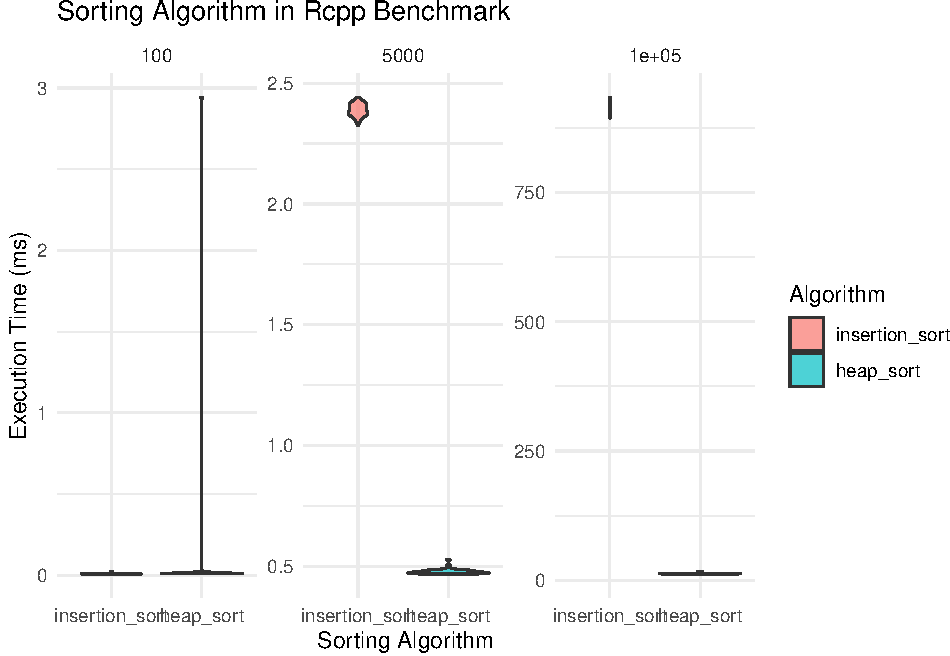
\includegraphics{1_Sorting_analyse_files/figure-latex/benchmark-1.pdf}

\begin{verbatim}
## # A tibble: 6 x 8
##        n expr            min_time q1_time median_time mean_time q3_time max_time
##    <dbl> <fct>              <dbl>   <dbl>       <dbl>     <dbl>   <dbl>    <dbl>
## 1    100 insertion_sort   0.00709 7.54e-3     0.00789   0.00846 8.76e-3   0.0207
## 2    100 heap_sort        0.00894 9.61e-3     0.00994   0.0692  1.05e-2   2.94  
## 3   5000 insertion_sort   2.32    2.37e+0     2.39      2.39    2.41e+0   2.44  
## 4   5000 heap_sort        0.468   4.71e-1     0.475     0.477   4.82e-1   0.527 
## 5 100000 insertion_sort 895.      9.08e+2   924.      919.      9.30e+2 935.    
## 6 100000 heap_sort       12.0     1.22e+1    12.3      12.4     1.23e+1  16.7
\end{verbatim}

\begin{center}\rule{0.5\linewidth}{0.5pt}\end{center}

\section{Evaluation de la
complexité}\label{evaluation-de-la-complexituxe9}

Les vecteurs de longueurs \texttt{vector\_n\_insertion} et
\texttt{vector\_n\_heap} (\texttt{n} dans les dataframes) sont choisis
sur l'echelle logarithmique afin d'avoir un pas constant sur l'échelle
logarithmique en abscisse pour la régression.

On réalise 10 répétitions pour chaque valeur de \texttt{n} et pour
chaque algorithme. Les barres d'erreur sont placées en ``mean +/- sd''.

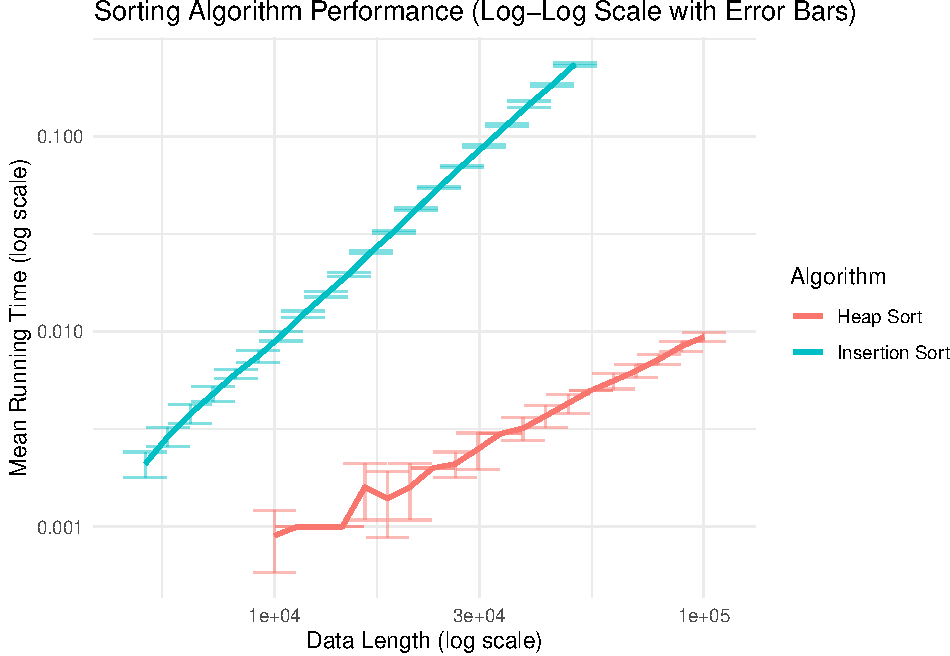
\includegraphics{1_Sorting_analyse_files/figure-latex/simu complexite-1.pdf}

\begin{Shaded}
\begin{Highlighting}[]
\NormalTok{res\_Heap}
\end{Highlighting}
\end{Shaded}

\begin{verbatim}
##         n mean_time      sd_time
## 1   10000    0.0009 3.162278e-04
## 2   11288    0.0010 4.493867e-15
## 3   12743    0.0010 7.338454e-15
## 4   14384    0.0010 4.493867e-15
## 5   16238    0.0016 5.163978e-04
## 6   18330    0.0014 5.163978e-04
## 7   20691    0.0016 5.163978e-04
## 8   23357    0.0020 6.864495e-15
## 9   26367    0.0021 3.162278e-04
## 10  29764    0.0025 5.270463e-04
## 11  33598    0.0030 0.000000e+00
## 12  37927    0.0032 4.216370e-04
## 13  42813    0.0037 4.830459e-04
## 14  48329    0.0043 4.830459e-04
## 15  54556    0.0050 7.338454e-15
## 16  61585    0.0056 5.163978e-04
## 17  69519    0.0063 4.830459e-04
## 18  78476    0.0072 4.216370e-04
## 19  88587    0.0084 5.163978e-04
## 20 100000    0.0094 5.163978e-04
\end{verbatim}

\begin{Shaded}
\begin{Highlighting}[]
\NormalTok{res\_Insertion}
\end{Highlighting}
\end{Shaded}

\begin{verbatim}
##        n mean_time      sd_time
## 1   5000    0.0021 0.0003162278
## 2   5644    0.0029 0.0003162278
## 3   6371    0.0038 0.0004216370
## 4   7192    0.0048 0.0004216370
## 5   8119    0.0061 0.0003162278
## 6   9165    0.0075 0.0005270463
## 7  10346    0.0095 0.0005270463
## 8  11679    0.0123 0.0004830459
## 9  13183    0.0156 0.0005163978
## 10 14882    0.0197 0.0004830459
## 11 16799    0.0257 0.0004830459
## 12 18963    0.0326 0.0005163978
## 13 21407    0.0424 0.0006992059
## 14 24165    0.0549 0.0007378648
## 15 27278    0.0705 0.0009718253
## 16 30792    0.0897 0.0014181365
## 17 34760    0.1148 0.0018135294
## 18 39238    0.1466 0.0059665736
## 19 44293    0.1838 0.0027406406
## 20 50000    0.2344 0.0041686662
\end{verbatim}

On vérifie la valeur du coefficient directeur pour les deux méthodes:

\begin{verbatim}
## 
## Call:
## lm(formula = log(res_Insertion$mean_time) ~ log(res_Insertion$n))
## 
## Residuals:
##       Min        1Q    Median        3Q       Max 
## -0.056330 -0.013396 -0.004171  0.013740  0.045334 
## 
## Coefficients:
##                        Estimate Std. Error t value Pr(>|t|)    
## (Intercept)          -23.381572   0.075886  -308.1   <2e-16 ***
## log(res_Insertion$n)   2.027908   0.007828   259.0   <2e-16 ***
## ---
## Signif. codes:  0 '***' 0.001 '**' 0.01 '*' 0.05 '.' 0.1 ' ' 1
## 
## Residual standard error: 0.02447 on 18 degrees of freedom
## Multiple R-squared:  0.9997, Adjusted R-squared:  0.9997 
## F-statistic: 6.711e+04 on 1 and 18 DF,  p-value: < 2.2e-16
\end{verbatim}

\begin{verbatim}
## Estimated exponent: 2.027908
\end{verbatim}

\begin{verbatim}
## 
## Call:
## lm(formula = log(res_Heap$mean_time) ~ log(res_Heap$n))
## 
## Residuals:
##       Min        1Q    Median        3Q       Max 
## -0.167735 -0.034582  0.005972  0.028454  0.173666 
## 
## Coefficients:
##                  Estimate Std. Error t value Pr(>|t|)    
## (Intercept)     -16.89548    0.25406  -66.50   <2e-16 ***
## log(res_Heap$n)   1.06075    0.02446   43.36   <2e-16 ***
## ---
## Signif. codes:  0 '***' 0.001 '**' 0.01 '*' 0.05 '.' 0.1 ' ' 1
## 
## Residual standard error: 0.07645 on 18 degrees of freedom
## Multiple R-squared:  0.9905, Adjusted R-squared:   0.99 
## F-statistic:  1880 on 1 and 18 DF,  p-value: < 2.2e-16
\end{verbatim}

\begin{verbatim}
## Estimated exponent: 1.060748
\end{verbatim}

Les coefficients dfirecteurs trouvés sont bien ceux que l'on attendait.
La valeur 2 pour l'insertion et 1 pour le tas.

\begin{center}\rule{0.5\linewidth}{0.5pt}\end{center}

\section{Cas particulier des données presque
triées}\label{cas-particulier-des-donnuxe9es-presque-triuxe9es}

On considère des données triées avec 5\% de valeurs échangées au hasard.

Sur un exemple cela donne :

\begin{Shaded}
\begin{Highlighting}[]
\NormalTok{v }\OtherTok{\textless{}{-}} \DecValTok{1}\SpecialCharTok{:}\DecValTok{100}
\NormalTok{n\_swap }\OtherTok{\textless{}{-}} \FunctionTok{floor}\NormalTok{(}\FloatTok{0.05} \SpecialCharTok{*} \FunctionTok{length}\NormalTok{(v))}
\NormalTok{swap\_indices }\OtherTok{\textless{}{-}} \FunctionTok{sample}\NormalTok{(}\FunctionTok{length}\NormalTok{(v), n\_swap)}
\NormalTok{v[swap\_indices] }\OtherTok{\textless{}{-}} \FunctionTok{sample}\NormalTok{(v[swap\_indices])}
\NormalTok{v}
\end{Highlighting}
\end{Shaded}

\begin{verbatim}
##   [1]   1   2   3   4   5   6   7   8   9  10  11  12  13  14  15  16  17  79
##  [19]  19  20  21  22  23  24  25  26  27  28  29  30  31  32  33  34  35  36
##  [37]  37  38  39  40  97  42  43  44  45  46  47  48  49  50  51  52  53  54
##  [55]  55  56  57  58  59  60  61  62  63  64  65  66  67  68  69  70  71  72
##  [73]  73  74  75  76  77  78  41  80  18  82  83  84  85  86  87  88  89  90
##  [91]  91  92  93  94  95  96  81  98  99 100
\end{verbatim}

\begin{Shaded}
\begin{Highlighting}[]
\NormalTok{one.simu2 }\OtherTok{\textless{}{-}} \ControlFlowTok{function}\NormalTok{(n, func)}
\NormalTok{\{}
\NormalTok{  v }\OtherTok{\textless{}{-}} \DecValTok{1}\SpecialCharTok{:}\NormalTok{n}
\NormalTok{  n\_swap }\OtherTok{\textless{}{-}} \FunctionTok{floor}\NormalTok{(}\FloatTok{0.05} \SpecialCharTok{*} \FunctionTok{length}\NormalTok{(v))}
\NormalTok{  swap\_indices }\OtherTok{\textless{}{-}} \FunctionTok{sample}\NormalTok{(}\FunctionTok{length}\NormalTok{(v), n\_swap)}
\NormalTok{  v[swap\_indices] }\OtherTok{\textless{}{-}} \FunctionTok{sample}\NormalTok{(v[swap\_indices])}
  \ControlFlowTok{if}\NormalTok{(func }\SpecialCharTok{==} \StringTok{"insertion\_sort"}\NormalTok{)\{}\FunctionTok{insertion\_sort}\NormalTok{(v)\}}
  \ControlFlowTok{if}\NormalTok{(func }\SpecialCharTok{==} \StringTok{"heap\_sort"}\NormalTok{)\{}\FunctionTok{heap\_sort}\NormalTok{(v)\} }
  \ControlFlowTok{if}\NormalTok{(func }\SpecialCharTok{==} \StringTok{"insertion\_sort\_Rcpp"}\NormalTok{)\{}\FunctionTok{insertion\_sort\_Rcpp}\NormalTok{(v)\}}
  \ControlFlowTok{if}\NormalTok{(func }\SpecialCharTok{==} \StringTok{"heap\_sort\_Rcpp"}\NormalTok{)\{}\FunctionTok{heap\_sort\_Rcpp}\NormalTok{(v)\}}
\NormalTok{\}}
\end{Highlighting}
\end{Shaded}

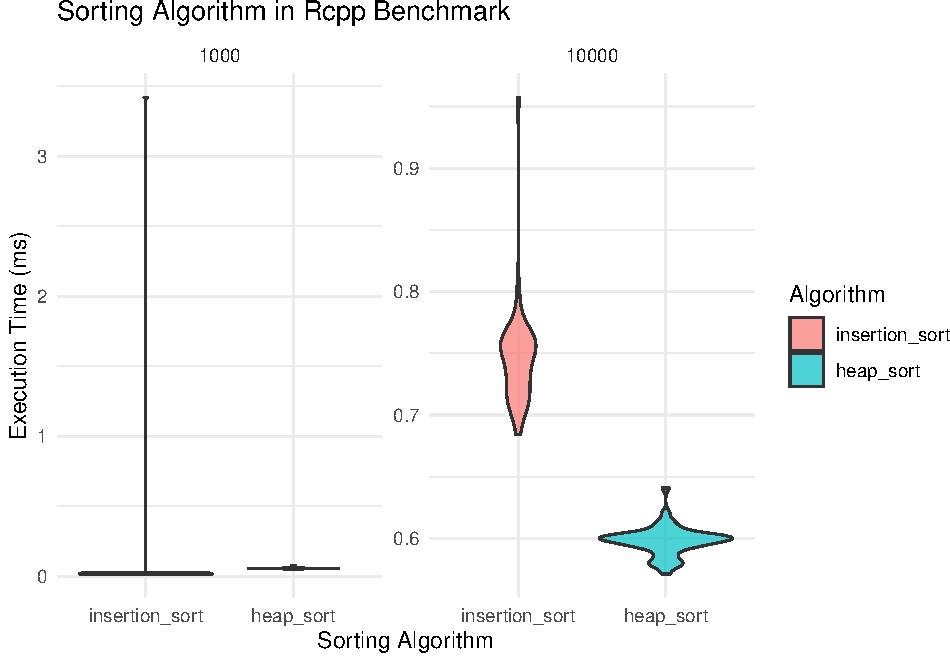
\includegraphics{1_Sorting_analyse_files/figure-latex/benchmark2-1.pdf}

\begin{verbatim}
## # A tibble: 4 x 8
##       n expr           min_time q1_time median_time mean_time q3_time max_time
##   <dbl> <fct>             <dbl>   <dbl>       <dbl>     <dbl>   <dbl>    <dbl>
## 1  1000 insertion_sort   0.0166  0.0178      0.0186    0.0868  0.0195   3.42  
## 2  1000 heap_sort        0.0516  0.0555      0.0568    0.0579  0.0579   0.0795
## 3 10000 insertion_sort   0.684   0.723       0.748     0.745   0.759    0.957 
## 4 10000 heap_sort        0.571   0.594       0.599     0.598   0.603    0.641
\end{verbatim}

L'algorithme d'insertion est ici plus rapide pour la longueur
\texttt{1000}. Cela est dû au fait que pour un vecteur déjà trié,
l'algorithme d'insertion est linéaire et nous sommes dans un cas proche
du linéaire.

\end{document}
